\chapter{Historia i wnioski}\label{ch:historia}

\begin{sekcja}{Skąd pochodzi platforma}
Zespół Stardust (Koło Naukowe SimLE, Politechnika Gdańska) wypuszcza balony stratosferyczne od 2016 roku. Pierwszą próbę startu zespół podjął w 2015 roku -- balon nie wzniósł się w powietrze (sekcja~\ref{sec:proba2015}). Pierwsze misje własne (2016--2020) służyły badaniom mikroorganizmów w stratosferze. W 2021 roku eksperyment Stardust poleciał na balonie BEXUS~30 w programie REXUS/BEXUS~\cite{iac2023,praca2022}. Po tym programie starsi członkowie skończyli studia. Nowy zespół, Stardust NEXT, zbudował małą platformę, którą może powtórzyć każdy nowy skład zespołu~\cite{pac2024}.

Praktyki projektowe z programu REXUS/BEXUS opisuje rozdział~\ref{ch:projekt}.

Po każdej misji dopisz wiersz do tabeli~\ref{tab:misje} i nowe wnioski do tabeli~\ref{tab:wnioski}.
\end{sekcja}

\begin{sekcja}{Misje własne}
\renewcommand{\arraystretch}{1.3}
\small
\begin{tabularx}{\linewidth}{@{}P{16mm}P{12mm}LP{12mm}P{36mm}P{15mm}@{}}
\toprule
\textbf{Data} & \textbf{Start} & \textbf{Ładunek} & \textbf{Pułap} & \textbf{Wynik} & \textbf{Źródła}\\\midrule
2015 & Polska & Pierwsza próba startu & -- & Start przerwany, balon nie poleciał. & relacja zespołu\\
26.04.2016 & Polska & Gondola ze styroduru, dwa moduły Arduino, odcinacz z drutem oporowym & -- & Pierwszy lot. Lądowanie na drzewie -- gondolę zdjęła straż pożarna podnośnikiem. & \cite{iac2023,stardustweb,dok2018}\\
27.09.2017 & Toruń & Układ próbkujący (test sterylności), odcinacz z drutem oporowym (zegar) & ok. 30 km & Balon pękł przed czasem odcięcia. Lądowanie przy małym cieku (Kotomierz). & \cite{magrian2018,iac2023,stardustweb}\\
05.2018 & Toruń & Układ próbkujący (2 filtry), grzałki, licznik Geigera, ładunek gościnny & 24,8 km & Sukces. & \cite{iac2023}\\
20.07.2020 & Toruń & Test układu dla BEXUS, ok. 4 kg, 2 gondole & 33,3 km & Brak odcinacza. Dryf 1,5 h. Lądowanie ok. 90 km od startu. & \cite{raport2020,praca2022}\\
27.02.2022 & Iława & Radiosonda z kamerą (lot szkoleniowy) & 33,4 km & Sukces. Lądowanie 51 km od startu, okolice Brodnicy. & \cite{blog2022,pac2024}\\
26.05.2023 & Iława & Platforma NEXT: OBC, łączność, odcinacz serwomechaniczny & 34 km & Odcinacz nie zadziałał. Lądowanie 23 km od startu. & \cite{blog2023,go2023,infoilawa2023,pac2024}\\
09.08.2023 & Polska & Platforma NEXT + ładunek STORM & -- & Odcinacz z drutem oporowym nie zadziałał. Ładunek zebrał dane. & \cite{pac2024,storm}\\
\midrule
\multicolumn{6}{@{}l}{\footnotesize\itshape Kolejne misje dopisuj poniżej:}\\[3mm]
\rule{0pt}{6mm} & & & & & \\\hline
\rule{0pt}{6mm} & & & & & \\\hline
\end{tabularx}
\captionof{table}{Misje balonowe zespołu Stardust. Źródła (artykuły, wpisy, media) -- w spisie literatury.}\label{tab:misje}
\end{sekcja}

\begin{sekcja}{Pierwsza próba (2015)}\label{sec:proba2015}
Pierwsza misja zespołu miała się odbyć w 2015 roku. Start był szeroko zapowiadany w mediach: było odliczanie, a nawet transmisja na żywo. Balon nie wzniósł się w powietrze i start się nie odbył.

Z tej próby zostały dwie lekcje:
\begin{enumerate}
  \item \textbf{Pierwsze próby zaczynają się od porażek.} Porażka jest częścią nauki i doskonalenia. Zapisz, co się stało, i popraw to w następnej misji.
  \item \textbf{Bezpieczeństwo przede wszystkim.} Przerwij start, gdy coś jest nie tak -- niezależnie od presji z zewnątrz: mediów, gości, sponsorów, transmisji na żywo.
\end{enumerate}
\begin{uwaga}Kierownik startu i kierownik misji mają prawo i obowiązek powiedzieć „no-go”. Zapowiedź w mediach nie jest powodem do startu.\end{uwaga}
\end{sekcja}

\begin{sekcja}{Pierwszy lot (26.04.2016)}
\noindent\begin{minipage}[t]{0.6\linewidth}\vspace{0pt}
Dokumentacja projektu~\cite{dok2018} opisuje platformę z pierwszych lotów (rysunki oznaczone rokiem 2016):
\begin{itemize}
  \item gondola ze styroduru (około $29\times29\times\SI{28}{cm}$), laminowana tkaniną szklaną \SI{48}{g/m^2} i żywicą epoksydową,
  \item balon lateksowy \SI{1200}{g}, około \SI{6}{m^3} helu; tankowanie trwało około 1,5 godziny,
  \item moduł A (Arduino Nano): czujniki ciśnienia, temperatury i wilgotności, GPS, zegar, karta SD,
  \item moduł B: próba stabilizacji obrotu gondoli kołem reakcyjnym oraz Bluetooth do sprawdzenia elektroniki tuż przed startem,
  \item odcinacz z drutem oporowym w obudowie drukowanej z ABS, krętlik nad odcinaczem.
\end{itemize}
Gondola wylądowała na drzewie. Zdjęła ją straż pożarna podnośnikiem (rysunek~\ref{fig:2016drzewo}).

Już wtedy zespół zauważył, że APRS bywa nieodbierany poniżej około \SI{200}{m}, i do poszukiwań używał trackera oraz ręcznego odbiornika APRS.
\end{minipage}\hfill
\begin{minipage}[t]{0.36\linewidth}\vspace{0pt}\centering
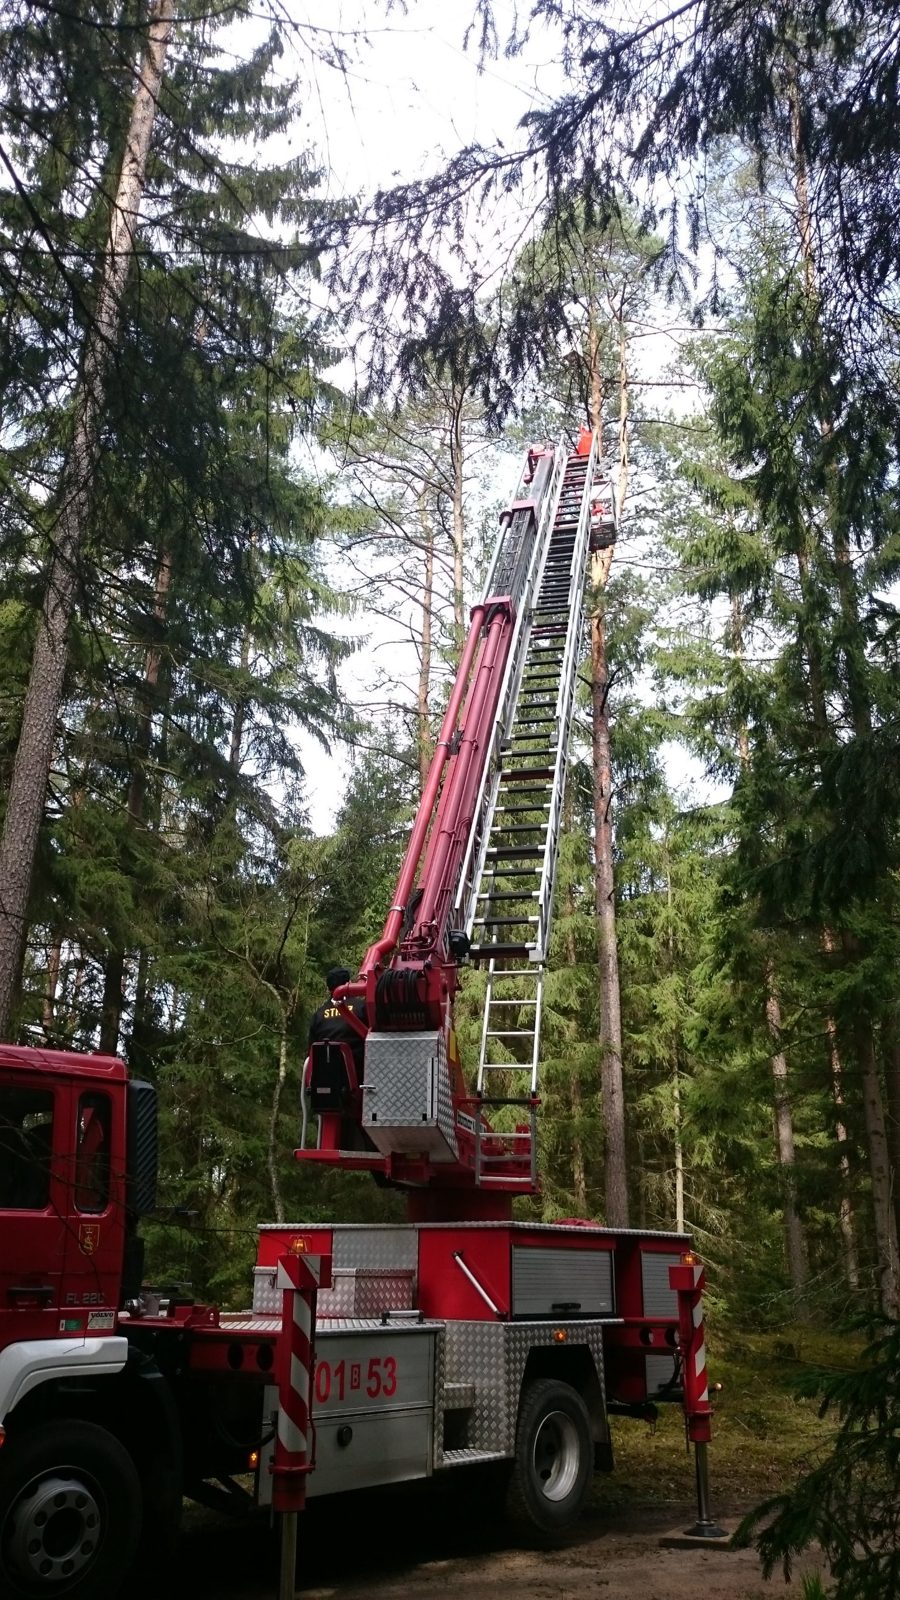
\includegraphics[width=\linewidth]{2016_gondola_drzewo_podnosnik}
\captionof{figure}{Gondola na drzewie po pierwszym locie (2016). Straż pożarna zdjęła ją podnośnikiem.}\label{fig:2016drzewo}
\end{minipage}
\end{sekcja}

\begin{sekcja}{Pierwsza misja mikrobiologiczna (27.09.2017)}
Lot testowy układu pobierającego próbki mikrobiologiczne, opisany w pracy inżynierskiej Szymona Magriana i Karola Pelznera~\cite{magrian2018}. Cel: sprawdzić sterylność układu i wszystkie podzespoły w stratosferze. Gondola ze styroduru z wkładką z plexi, masa \SI{2.6}{kg}, balon Hwoyee \SI{1600}{g}, hel, spadochron okrągły \SI{1}{m}. Start z Torunia o 10:06~UTC, lądowanie o 12:08~UTC.

Co się wydarzyło i czego to uczy:
\begin{itemize}
  \item \textbf{Odcinacz z drutem oporowym działał według zegara.} Czas odcięcia (11:30~UTC) wynikał z predykcji. Balon wznosił się szybciej i pękł wcześniej (11:24~UTC). Drut się rozgrzał, ale bez naciągu linki nie przepalił jej. Wniosek: drut oporowy przecina linkę tylko pod obciążeniem, a odcinacz powinien działać według wysokości, nie tylko zegara.
  \item \textbf{Usterki elektroniki:} karta SD wypadła z gniazda od wstrząsów (zapis tylko z pierwszych 30 minut), przewód czujnika ciśnienia urwał się przy starcie, część czujników nie zapisała danych. Przyczyna: płytka prototypowa i słabe mocowania. Wniosek: płytka PCB, pewne mocowania, test wstrząsów i diody stanu do kontroli przed startem.
  \item \textbf{Kamery} przesunęły się w czasie przygotowań -- część obrazu zasłonił styrodur. Wniosek: sprawdź kadr tuż przed zamknięciem gondoli.
  \item \textbf{Odzyskanie:} ostatnia pozycja APRS pochodziła z wysokości \SI{167}{m}. Gondolę znalazł zespół dzięki telefonowi w gondoli i brzęczykowi (wysoka trawa). Gondola wylądowała około \SI{3}{m} od małego kanału -- gondola musi pływać.
  \item \textbf{Spadochron:} średnia prędkość opadania poniżej \SI{2.8}{km} wyniosła \SI{5.45}{m/s} dla \SI{2.6}{kg} i spadochronu \SI{1}{m}.
\end{itemize}
\end{sekcja}

\begin{sekcja}{Misja mikrobiologiczna (2018)}
Ładunek z grzaną sekcją na komórki, pompą i licznikiem Geigera. Dane z rejestratora pokładowego i z APRS pokazuje rysunek~\ref{fig:misja2018}.

\begin{center}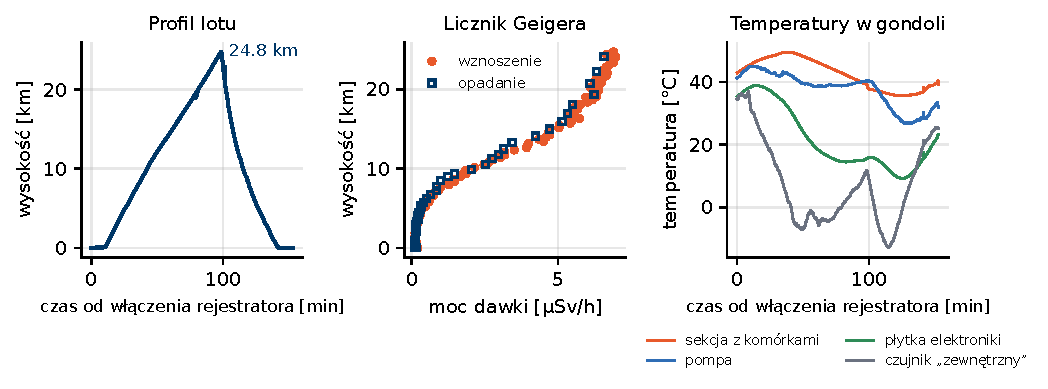
\includegraphics[width=\linewidth]{misja_2018}\end{center}
\captionof{figure}{Misja mikrobiologiczna z 2018 roku (okolice Torunia): profil lotu, moc dawki z licznika Geigera i temperatury w gondoli. Dane: \texttt{data/2018\_mikrobiologia\_*.csv}.}\label{fig:misja2018}

\begin{itemize}
  \item Pułap \SI{24.8}{km}. Moc dawki rosła z wysokością: od około \SI{0.13}{\micro Sv/h} przy ziemi do około \SI{7}{\micro Sv/h} na \SI{23}{}--\SI{25}{km}.
  \item Grzałki utrzymały sekcję z komórkami w zakresie 36--\SI{50}{\degreeCelsius}. Płytka elektroniki ochłodziła się do około \SI{9}{\degreeCelsius}.
  \item Czujnik opisany jako „zewnętrzny” pokazał minimum \SI{-13}{\degreeCelsius}, a powietrze na wysokości 10--\SI{12}{km} ma około \SI{-50}{\degreeCelsius}. Czujnik mierzył ściankę gondoli, nie powietrze. Wniosek: czujnik temperatury powietrza musi wystawać z gondoli i mieć osłonę przed słońcem.
  \item Czujnik ciśnienia nie podawał wartości powyżej około \SI{18}{km} (\SI{52}{hPa}). Sprawdź zakres czujnika w karcie katalogowej.
\end{itemize}
\end{sekcja}

\begin{sekcja}{Trasy lotów}
Rysunek~\ref{fig:mapa} pokazuje trasy lotów z dostępnymi danymi. Przy wietrze z zachodu balon leci na wschód -- w stronę granicy z Rosją (obwód królewiecki) i Białorusią. Predykcja trajektorii jest więc warunkiem każdego startu (rozdział~\ref{ch:planowanie}).

\begin{center}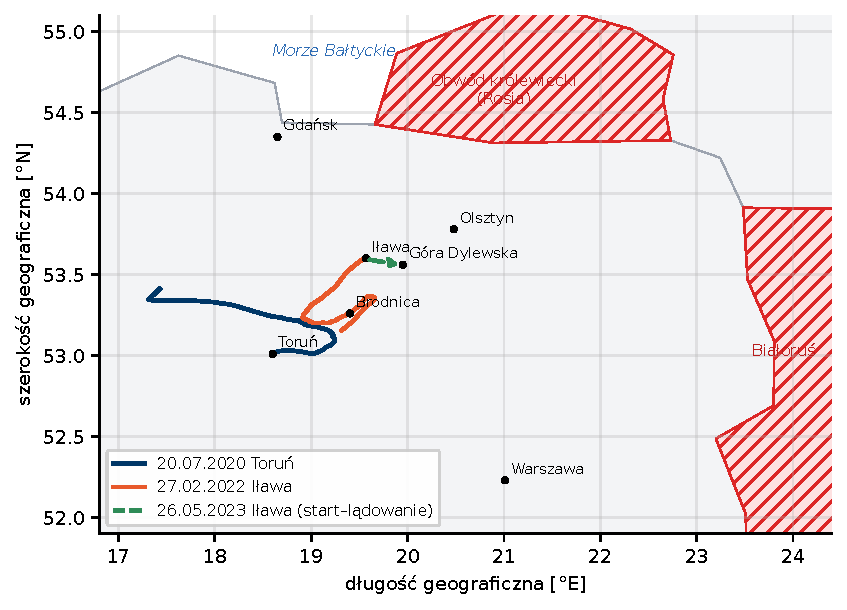
\includegraphics[width=0.92\linewidth]{mapa_lotow}\end{center}
\captionof{figure}{Trasy lotów z lat 2020--2023. Kreskowane obszary: państwa, nad którymi lot i lądowanie są niedopuszczalne.}\label{fig:mapa}
\end{sekcja}

\begin{sekcja}{Profil lotu w przestrzeni}
\begin{center}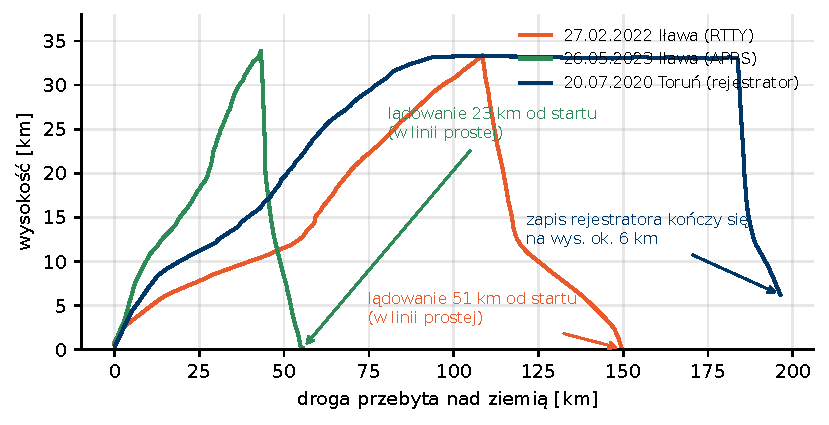
\includegraphics[width=\linewidth]{profil_dystans}\end{center}
\captionof{figure}{Wysokość w funkcji drogi przebytej nad ziemią. Dane z trackera (2022) i z rejestratora pokładowego (2020).}\label{fig:profil-dystans}

\foto[\linewidth]{2022_profil_lotu_2022_google_earth}{Profil misji z 27.02.2022 w Google Earth. Po prawej Zatoka Gdańska.}
\end{sekcja}

\begin{sekcja}{Lot szkoleniowy (27.02.2022)}
Cel: nauczyć nowy zespół procedur. Ładunek: radiosonda z kamerą, telemetria RTTY i APRS pod znakiem SR0FLY (SR0FLY-12), użytym za zgodą jego właściciela (rozdział~\ref{ch:prawo}).

Zespół ćwiczył trzy fazy:
\begin{enumerate}
  \item przygotowanie sprzętu i stanowiska startowego,
  \item tankowanie i start,
  \item śledzenie, pościg samochodem, odzyskanie.
\end{enumerate}

\begin{wskazowka}Ten format to wzór dla każdej nowej grupy: pierwsza misja ma prosty ładunek i skupia się na procedurach.\end{wskazowka}

\dwafoto{2022_stanowisko_zabezpieczone}{Stanowisko startowe: plandeka i folia dociśnięte skrzynkami (27.02.2022).}
{2022_poscig_samochod}{Pościg: laptop z mapą śledzenia i radiotelefon w samochodzie (27.02.2022).}
\end{sekcja}

\begin{sekcja}{Test platformy (26.05.2023)}
Pierwsza misja, którą nowy zespół zaprojektował i zbudował samodzielnie. Testowane systemy: komputer pokładowy (OBC), łączność i namierzanie, olinowanie z odcinaczem mechanicznym, gondola z pudełek styropianowych. Lot: \SI{34}{km} po około 90 minutach, lądowanie w okolicy Góry Dylewskiej~\cite{blog2023}.

Odcinacz był w gondoli, nie pod balonem. Powód: zespół nie miał doświadczenia z odcinaczem sterowanym zdalnie pod powłoką. Serwo w gondoli miało zwolnić linkę, która trzyma balon.

\textbf{Problem:} odcinacz nie zadziałał. Gondola obracała się w locie. Krętlik był tylko na górze olinowania. Na dole linki skręciły się i linka odcinacza nie mogła się zwolnić~\cite{pac2024}.

\textbf{Zabezpieczenie, które zadziałało:} zapas 10--15~m linki odcinacza między krętlikiem a spadochronem. Spadochron miał miejsce na rozwinięcie mimo skręconych linek. Zestaw wylądował bezpiecznie.

\foto[0.7\linewidth]{2020_odzysk_resztki_powloki}{Po lądowaniu: resztki pękniętej powłoki i gondola (20.07.2020).}
\end{sekcja}

\begin{sekcja}{Ładunek STORM (09.08.2023)}
Pierwsza misja nowego zespołu bez pomocy starszych członków. Zespół zmniejszył masę komponentów i zastąpił odcinacz serwomechaniczny odcinaczem z drutem oporowym. Olinowanie bez zmian.

\textbf{Problem:} drut oporowy grzał się za krótko i nie przeciął linki~\cite{pac2024}.
\end{sekcja}

\clearpage
\section{Wnioski}
Stosuj te wnioski w każdej misji.

\renewcommand{\arraystretch}{1.3}
\begin{longtable}{@{}P{27mm}>{\raggedright\arraybackslash}p{0.62\linewidth}P{12mm}@{}}
\toprule
\textbf{Obszar} & \textbf{Wniosek} & \textbf{Misja}\\\midrule\endhead
\bottomrule\endfoot
Odcinacz & Każdy lot musi mieć odcinacz. Bez odcinacza balon może dryfować godzinami i wylądować daleko. & 2020\\
Odcinacz & Testuj odcinacz w warunkach lotu: zimno, obrót gondoli, skręcone linki, pełne obciążenie. Daj drugi, niezależny odcinacz innego typu. & 2023\\
Odcinacz & Drut oporowy musi dostać prąd wystarczający do przecięcia linki. Sprawdź to z docelowym tranzystorem i baterią, wiele razy i w zimnie. & 2023\\
Olinowanie & Gondola obraca się w locie. Daj krętlik pod balonem i zapas linki odcinacza nad spadochronem. Poprzeczki na linkach mogą ograniczyć skręcanie (do sprawdzenia kamerą w locie). Długość zapasu to wciąż eksperyment: próbuj krótszej i zapisz wynik. & 2023\\
Gaz & Butla może mieć mniej gazu, niż deklaruje dostawca. Zamów gaz z zapasem. Mierz siłę nośną obciążnikiem. & 2020\\
Wysokość & Wzór na wysokość z ciśnienia działa tylko do około 10~km. Powyżej używaj GPS. & 2020\\
Czujniki & Czujnik BME280 nie mierzy poniżej \SI{300}{hPa}. Odrzucaj kody błędów czujników w programie. & 2020\\
Anteny & Źle zmontowana antena wyłączyła APRS. Sprawdzaj odbiór z odległości co najmniej \SI{100}{m}. & 2020\\
Śledzenie & Używaj co najmniej dwóch niezależnych systemów śledzenia i lokalizatorów po lądowaniu. & 2020\\
Łączność wewn. & Nie używaj WiFi między gondolami. Używaj kabla albo osobnego GPS w każdej gondoli. & 2020\\
Zasilanie & Każde urządzenie (także kamera) musi działać przez cały lot z zapasem. Kamera bez zewnętrznej baterii wyłączyła się po 30 minutach. & 2020\\
Termika & Elektronika w izolowanej gondoli może się przegrzać latem (ponad \SI{50}{\degreeCelsius}). & 2020\\
Mechanika & Mocuj elektronikę na wkładce. Dystanse PCB pękły przy lądowaniu. & 2020\\
Montaż & Każdy podzespół ma osobę odpowiedzialną albo opisaną procedurę montażu. & 2020\\
Diagnostyka & Dodaj diody statusu, aby szybko sprawdzić stan systemu na stanowisku. & 2020\\
Planowanie & Wiatr decyduje o trasie lotu. Planuj start z predykcją trajektorii. & 2016\\
Bezpieczeństwo & Przerwij start, gdy coś jest nie tak -- niezależnie od presji mediów, gości i sponsorów. Porażka jest częścią nauki. & 2015\\
Odcinacz & Drut oporowy przecina linkę tylko pod obciążeniem: po pęknięciu balonu nie przetnie. Odcinaj według wysokości, nie tylko zegara. & 2017\\
Mechanika & Karta SD wypadła z gniazda od wstrząsów, przewody urwały się przy starcie. Używaj PCB i pewnych mocowań, testuj wstrząsy. & 2017\\
Kamery & Kamera przesunęła się w czasie przygotowań. Sprawdź kadr tuż przed zamknięciem gondoli. & 2017\\
Odzyskanie & Gondola może zawisnąć na drzewie. Przygotuj kontakt do arborysty albo firmy z podnośnikiem. & 2016\\
Odzyskanie & Ostatnia pozycja APRS bywa z wysokości kilkuset metrów. Telefon albo lokalizator w gondoli i brzęczyk pozwalają znaleźć gondolę. & 2017\\
Gondola & Gondola musi pływać i być szczelna. Sprawdź ją w wannie z wodą, z obciążeniem do docelowej masy. & 2017\\
Czujniki & Czujnik temperatury powietrza musi wystawać z gondoli i mieć osłonę przed słońcem. Sprawdź zakres czujnika ciśnienia. & 2018\\
Zespół & Pierwsza misja nowego zespołu to lot szkoleniowy z prostym ładunkiem. & 2022\\
% Puste wiersze dopełniają stronę na nowe wnioski.
\rule{0pt}{7mm} & & \\\hline
\rule{0pt}{7mm} & & \\\hline
\rule{0pt}{7mm} & & \\\hline
\rule{0pt}{7mm} & & \\\hline
\rule{0pt}{7mm} & & \\\hline
\rule{0pt}{7mm} & & \\\hline
\rule{0pt}{7mm} & & \\\hline
\rule{0pt}{7mm} & & \\\hline
\rule{0pt}{7mm} & & \\\hline
\rule{0pt}{7mm} & & \\\hline
\rule{0pt}{7mm} & & \\\hline
\rule{0pt}{7mm} & & \\\hline
\rule{0pt}{7mm} & & \\\hline
\rule{0pt}{7mm} & & \\\hline
\rule{0pt}{7mm} & & \\\hline
\rule{0pt}{7mm} & & \\\hline
\rule{0pt}{7mm} & & \\\hline
\rule{0pt}{7mm} & & \\\hline
\rule{0pt}{7mm} & & \\\hline
\rule{0pt}{7mm} & & \\\hline
\rule{0pt}{7mm} & & \\\hline
\rule{0pt}{7mm} & & \\\hline
\rule{0pt}{7mm} & & \\\hline
\rule{0pt}{7mm} & & \\\hline
\rule{0pt}{7mm} & & \\\hline
\rule{0pt}{7mm} & & \\\hline
\rule{0pt}{7mm} & & \\\hline
\rule{0pt}{7mm} & & \\\hline
\rule{0pt}{7mm} & & \\\hline
\rule{0pt}{7mm} & & \\\hline
\rule{0pt}{7mm} & & \\\hline
\rule{0pt}{7mm} & & \\\hline
\rule{0pt}{7mm} & & \\\hline
\rule{0pt}{7mm} & & \\\hline
\rule{0pt}{7mm} & & \\\hline
\rule{0pt}{7mm} & & \\\hline
\rule{0pt}{7mm} & & \\\hline
\caption{Wnioski z poprzednich misji. Puste wiersze na nowe wnioski.}\label{tab:wnioski}
\end{longtable}
